\documentclass[12pt,oneside,a4paper]{article} % for sharing
\usepackage{apacite}
\usepackage{appendix}
\usepackage{amsmath}
\usepackage{amsthm}
\usepackage{multirow}
\usepackage{amssymb} % for approx greater than
\usepackage{caption}
\usepackage{placeins} % for \FloatBarrier
\usepackage{graphicx}
\usepackage{subcaption}
\usepackage{longtable}
\usepackage{setspace}
\usepackage{booktabs}
\usepackage{tabularx}
\usepackage{xcolor,colortbl}
\usepackage{chngpage}
\usepackage{natbib}
\bibpunct{(}{)}{,}{a}{}{;} 
\usepackage{url}
\usepackage{nth}
\usepackage{authblk}
\usepackage[most]{tcolorbox}
\usepackage[normalem]{ulem}
\usepackage{amsfonts}

% scraped out necessary stuff from hal's loghead file

% new commands defined

%bold faced letters
\newcommand{\bo}[1]{{\bf #1}}

\newcommand{\bm}[1]{\mbox{\boldmath $#1$}}
\newcommand{\kron}{\otimes}
\renewcommand{\vec}{\mbox{vec} \,}

%begin and end equations
\newcommand{\be}{\begin{equation}}
\newcommand{\ee}{\end{equation}}

%begin and end equations without numbers
\newcommand{\bd}{\begin{displaymath}}
\newcommand{\ed}{\end{displaymath}}

%begin and end equation arrays
\newcommand{\bea}{\begin{eqnarray}}
\newcommand{\eea}{\end{eqnarray}}

%begin and end equation arrays without numbers
\newcommand{\beastar}{\begin{eqnarray*}}
\newcommand{\eeastar}{\end{eqnarray*}}

%begin and end matrices
\newcommand{\bmat}[1]{\left(\begin{array}{#1}}
\newcommand{\emat}{\end{array}\right)}

%equation numbers
\newcommand{\enum}[1]{\label{eq:#1}}

%derivatives and elasticities
\newcommand{\der}[2]{{d #1 \over d #2}}
\newcommand{\elas}[2]{{\varepsilon #1 \over \varepsilon #2}}


%partial derivatives and second partial derivatives
\newcommand{\pder}[2]{{\partial #1 \over \partial #2}}
\newcommand{\secpderij}[3]{{\partial^2 #1 \over \partial #2 
            \partial #3}}
\newcommand{\tsecpderij}[3]{\partial^2 #1 / \partial #2 
            \partial #3}  %text second partial

\newcommand{\secpderii}[2]{{\partial^2 #1 \over \partial #2^2}}
\newcommand{\tsecpderii}[2]{\partial^2 #1 / \partial #2^2}
%   text second partial

%matrix transpose symbol
\newcommand{\tr}{{\mbox{\tiny \sf T}}}

%matrix diagonal symbol
%\newcommand{\diag}{\mbox{diag} \,}
\newcommand{\diag}{\mathcal{D}}

\newcommand{\trace}{\mbox{trace}}

\newcommand{\dg}{{\rm{dg}}}

% \mc{number of columns}{position}{item}
\newcommand{\mc}[3]{\multicolumn{#1}{#2}{#3}}
% center a single item in a table
\newcommand{\cent}[1]{\mc{1}{c}{#1}}

\newcommand{\mcal}[1]{\mathcal{#1}}


\newcommand{\str}[1]{\rule{0in}{#1}}
\newcommand{\tbar}[1]{\left. \rule{0in}{#1} \right|}





\newcommand{\rind}{\noindent\hangindent=20pt\hangafter=1}

%%%%%%%%%
% margin adjustments
% these are for US letter size paper; should be adjusted for A4
%%%%%%%%

\textwidth=6.5in
 \oddsidemargin=0in
 %\evensidemargin=0.125in
 %\evensidemargin=0.5in
 \textheight=9.0in
 \topmargin=0.0in
 \headheight=0.0in
 \headsep=0.0in

%%%%%%%%%%%%
% end of margin adjustments
%%%%%%%%%%%% 

%%%%%% stuff from here on not used much %%%%%

% \newtheorem{theorem}{Theorem}[section]
%\newtheorem{theorem}{Theorem}

%\newtheorem{example}{Example}[section]
\newtheorem{example}{Example}

    \newcommand{\exbegin}[1]{\begin{itemize} \item[~]

    \begin{example}{\bf #1} \begin{rm} }
    \newcommand{\exend}{\end{rm}\end{example}
    \end{itemize}}
\newcommand{\scp}[1]{\langle #1 \rangle}
\setcounter{secnumdepth}{3}
\setcounter{tocdepth}{4}

\newtheorem{newfig}{Figure}
\newcommand{\figbegin}{\begin{newfig} \begin{rm} }
\newcommand{\figend}{\end{rm} \end{newfig}}
% commands to change float restrictions
\renewcommand{\topfraction}{0.99}
\renewcommand{\bottomfraction}{0.99}
\renewcommand{\textfraction}{0}
\renewcommand{\floatpagefraction}{0}

\newcommand{\mathbold}[1]{\mbox{\boldmath $\bf#1$}}
% Shultis, Latex Notes, p. 54


%Commands for biblist
\newenvironment{biblist}{\begin{list}{}{\setlength{\leftmargin}{0.15in}% 
\setlength{\itemindent}{-0.15in} \setlength{\parsep}{0.in}%
\setlength{\itemsep}{0.1in}}}{\end{list}} 

% columns for longtable
\newcolumntype{C}[1]{>{\centering\let\newline\\\arraybackslash\hspace{0pt}}m{#1}}
\newcolumntype{L}[1]{>{\raggedright\let\newline\\\arraybackslash\hspace{0pt}}m{#1}}
\usepackage{arydshln} % Dashed lines in matrices


\usepackage[margin=1in]{geometry}
%\doublespacing % for review

% line numbers to make review easier
%\usepackage{lineno}
%\linenumbers

%\usepackage{soul}% for \st{}

%%%%%%%%%%%%%%%%%%%%%%%%%%%%%%%%%%%%%%%%%%%%%%%%%%%%%%%%%%%%%%%%%%%%%%%%%%%%%%
% for section 4 math environments
\theoremstyle{definition}
\newtheorem{definition}{Definition}[section]
\newtheorem{theorem}{Theorem}[section]
\newtheorem{proposition}{Proposition}[section]
\newtheorem{corollary}{Corollary}[proposition]
\newtheorem{remark}{Remark}[section]

%%%%%%%%%%%%%%%%%%%%%%%%%%%%%%%%%%%%%%%%%%%%%%%%%%%%%%%%%%%%%%%%%%%%%%%%%%%%%%

\newcommand\ackn[1]{%
  \begingroup
  \renewcommand\thefootnote{}\footnote{#1}%
  \addtocounter{footnote}{-1}%
  \endgroup
}

% Affiliations in small font size
\renewcommand\Affilfont{\small}

\defcitealias{HMD}{HMD 2016}

% junk for longtable caption
\AtBeginEnvironment{longtable}{\linespread{1}\selectfont}
\setlength{\LTcapwidth}{\linewidth}

% sort van Raalte properly
% #1: sorting key, #2: prefix for citation, #3: prefix for bibliography
\DeclareRobustCommand{\VAN}[3]{#2} % set up for citation

%%%%%%%%%%%%%%%%%%%%%%%%%%%%%%%
\begin{document}


\title{The changing contribution of socioeconomic deprivation to variance in age at death}
%\author{author(s) redacted}
\author[1]{Rosie Seaman\thanks{seaman@demogr.mpg.de}}
\author[1]{Tim Riffe}
\author[2]{Hal Caswell}

\affil[1]{Max Planck Institute for Demographic Research, Rostock, Germany}
\affil[2]{University of Amsterdam, Netherlands}

\maketitle

\begin{abstract}
Mortality inequalities demonstrate a double burden: the most deprived socioeconomic
groups experience the lowest average age of death and the highest variation in
age at death. Two processes generate variation in age at death: individual
stochasticity (within-group variance) and heterogeneity (between-group
inequality). Limited research has evaluated how these two components have
changed over time. We address this research gap by using population and
mortality data for the entire population of Scotland stratified by area-level deprivation for 1981-2011. The most deprived areas have experienced stagnating or slight increasing variance in
age at death and the least deprived areas have experienced decreasing variance.
This is consistent with the literature demonstrating that there is not
simply a social gradient for variation in age at death but that socioeconomic groups have experienced diverging trends. The relative contributions from between-group inequality increased faster than than the relative inequalities from within-group inequality, indicating that area-level deprivation may be increasingly important for total variation in age at death.
\end{abstract}

\section{Background}
The relationship between socioeconomic inequality and mortality is traditionally
based on life expectancy comparisons. The most deprived populations
experience the lowest average age of death, and the least deprived populations
experience the highest. Studies have further demonstrated that the most deprived
populations also demonstrate the highest level of variation in age at death when
measuring socioeconomic inequality by income, education, or occupation
\citep{Broennum-Hansen2017,Raalte2011,Sasson2016,Raalte2014}. Higher variation in age at death means greater uncertainty leading to the notion that the social patterning of these two distinct dimensions of mortality is a double burden of inequality. 

Homogeneity in age at death is desirable for both individuals and societies in terms of forecasting pensions, comparing savings and investments, and estimating health care and social security needs \citep{Raalte2011}. Relatively low and decreasing variation also
means that the risk of premature death is being reduced for the population\footnote{increasing variation comes from both
premature deaths and deaths at very old ages, and theoretically the latter could
drive increasing variance, but this is not the case for Scotland or any of its
deprivation quantiles}. Greater reductions in the risk of premature death may be a feature of population mortality associated with more efficient social security systems and higher welfare redistribution 
\citep{Raalte2012,Bambra2011,Popham2013}. Despite the growing body of evidence documenting the double burden of mortality inequality variation in age at death is not yet routinely measured alongside life expectancy. This is important for evaluating the extent to which public health policies are simultaneously improving average mortality and reducing inequalities (N\'emeth \citeyear{Nemeth2017}, Smits and Monden \citeyear{Smits2009}).
  
Two processes underly the total variance in age at death: individual
stochasticity (within-group variance) and heterogeneity (between-group
inequality). Within-group variance tends to arise from differences due to random
demographic processes. The lifetable assumes that every individual, at the same age, is subject
to the same schedule of mortality rates, such that any
variance in age of death can be interpreted as individual stochasticity.
Within-group variance can also be due to unaccounted for subgroup heterogeneity.
For example males and females have different mortality schedules. Aggregating
a lifetable over both sexes increases within-group variance due to induced
between-group heterogeneity, even if males and females have identical
within-group variance. It is also possible that a lifetable could be produced for populations that are
heterogeneous but without knowing the reasons why the mortality of the populations are disparate and being unable to produce stratified lifetables. Therefore, within-group variance is theoretically always inflated
due to heterogeneity on unmeasured characteristics of the population. For
example, we cannot always stratify our lifetables on all characteristics that are hypothesized to be important for mortality such as marital, employment, or diabetes status: characteristics of a population that are likely to account for a
non-trivial fraction of within-group variance.


Between-group lifespan inequality arises when individuals at the same age are
subject to different mortality rates, which may be due to exposures to
different social, economic, or environmental contexts \citep{Hartemink2017}.
\citet{Raalte2012} estimated the contribution of educational inequalities (the
between-group component) to the total variance in age at death for 11 individual European countries. For males in Sweden the between-group component accounted for 1.7\% of the total variance in age at death but for males in the Czech Republic it accounted for 10.9\% of total variance in age at death. The between-group component was higher in the Czech Republic because the age distributions of death, stratified by education, are more disparate than in Sweden. 
%Noted was the distinct age distribution for the least educated males in the
% Czech Republic. 
\citet{Raalte2012} used data aggregated over 1990 to 2000, such
that time trends for the between-group and within-group components could not be assessed. 
% check- is that in said paper, ir did it come from Hendi?
In addition, it recognised that education may be a problematic socioeconomic
measure for studying trends in between-group components due to
changes in educational composition and the meanining of education attainment
\citep{Raalte2012,Hendi2015}.
A further limitation when stratifying data by education is that researchers
may need to left-truncate data at some age, that may not be consistent across time or across comparison countries, because education is acquired
over the life course. 
%(although
%\citet{Broennum-Hansen2017} used an indicator of disposable household income
%that does not require age truncation, results were still reported as age
% conditional).
Area-level measures of relative deprivation have tended to be used as simple proxy measures for individual or household level socioeconomic indicators. They are able to overcome the limitations of education and social class indicators which are poorly recorded, or even absent, for large groups of the population \citep{Morgan2006}.  However, it is now recognized that area-level deprivation can have an influence on risk of death independent of individual level socioeconomic circumstance \citep{Carstairs1989,Macintyre2002,Tunstall2011}. Empirical results are somewhat mixed but it remains valuable to understand that mortality outcomes are not only driven by characteristics of individuals but also by the collective and contextual characteristics of areas \citep{Macintyre2002}. 

It is important to recognize that choice of area-level measure will be driven by conceptual and pragmatic factors. However, most aim to capture the notion of relative deprivation in order to understand its impact on health \citep{kearns2000,Morgan2006}. Relative deprivation is the concept that not having enough material cultural
or social resources to participate in the socially accepted way of life is as important for health as absolute poverty \citep{Townsend1987,Carstairs1989,Kearns2000,Kawachi2002}. This hypothesis is supported by studies showing that more equal societies have better health outcomes, even if the material standards of living are worse in absolute terms \citep{Wilkinson1997,Marmot2001,Wilkinson2007}. In pragmatic terms, area-level measures of relative deprivation tend to weight equal sized population groups into quantiles. This gives a
consistent interpretation over time; although
absolute levels of poverty in a country will have changed there is a notional
most deprived fraction of the population being compared with a notional least deprived fraction of the same size. 
Area-level measures constructed from administrative data have a practical advantage over area-level measures constructed from survey data because they can be updated more frequently. Assigning individuals to an area-level measure deprivation based on their post-code is also advantageous. Left age truncation is not required because home
address is routinely collected across all stages of the life course and
passively by a range services, while measures of income, occupation,
or education again tend to be derived from survey data and are age dependent characteristics.

We contribute to the mortality inequalities literature by measuring the changing contributions from within and
between-group components to variance in age at death. Data are centered on
Census years, ensuring the most robust population estimates available.
Populations in each postal code are aggregated base on population-weighted
quintiles of the Carstairs score distribution. Death counts are
matched to postal codes based on place of usual residence and then aggregated
on Carstairs quintiles. The data include the whole population of Scotland (ca 5
million persons) and cover the time period between 1981 and 2011.

\section{Data and methods}

\subsection{Area-level deprivation}
Census population estimates and mortality data\footnote{Mortality data used
came from 1980-1982, 1990-1991, 2000-2002 and 2010-2012 to increase the
number of events centered around each census. 1990-1991 is just a two-year
numerator sample due to geographical boundary changes occurring in 1990.
Corresponding Census population estimates are adjusted accordingly.} by single
year of age and sex for each part-postcode (zip-code) sector in Scotland were
obtained via a commissioned request to National Records of Scotland. There are
around 1,012 part-postcode sectors in Scotland at each Census year each with an
average population size of 5,000 individuals. Table~\ref{tab:PCsect} shows the number of postcode sectors and the population sizes for each Census year.

% Table generated by Excel2LaTeX from sheet 'Sheet1'
\begin{table}[htbp]
  \centering
    \label{tab:PCsect}
  \caption{Number of postcode sectors and population size}
    \begin{tabular}{rrrr}
    \multicolumn{1}{l}{Year} & \multicolumn{1}{l}{Number} & \multicolumn{1}{l}{Mean pop.} & \multicolumn{1}{l}{sd} \\
    \midrule

    1981  & 1010  & 4982.47 & 1178.53 \\
    1991  & 1001  & 4993.02 & 1653.67 \\
    2001  & 1010  & 5011.89 & 1542.42 \\
    2011  & 1012  & 5232.61 & 1568.05 \\
    \bottomrule
    \end{tabular}%
  \label{tab:addlabel}%
\end{table}%


 
Population-weighted quintiles (each 20\% of the population) were created by
aggregating the 1,012 part-postcode sectors ordered on Carstairs score of
deprivation. The Carstairs score is a z-score for each part-postcode sector
that is derived from four individual-level census variables: overcrowding, male
unemployment, low social class, and car ownership. The Carstairs Score
(z-score) reflects the material resources that provide the means to access the
goods, services, amenities, and physical environment seen as expected
in society \citep{Carstairs1989}. This means the Carstairs score is a method of
capturing relative deprivation at the contextual level (cite). In 2011 for example, scores ranged from -7.53 to 13.24 and were centered on zero, with higher scores indicating relatively higher deprivation than the national level.

\subsection{Lifetables and variance decomposition}
Deaths\footnote{NRS policy for assigning geography to each death - deaths of Scottish residents that occur in Scotland are assigned to their place of normal residence, deaths of non-Scottish residents that occur in Scotland are assigned a geography based on their place of death, deaths of Scottish residents that occur outside of Scotland are not included\citep{GeneralRegisterOfficeforScotland2016}} and Census population denominators were used to construct complete
lifetables for each deprivation quintile, centered on each Census year, for
males and females separately.  The Human Mortality Database
Methods Protocol was used to extrapolate age specific mortality rates from
ages 85 to 110 \citep{Wilmoth2017}.\footnote{Specifically, we apply equations (53) and
(54) from the HMD protocol v6, modified to use information from ages 75+
rather than 80+.} 

From the complete lifetables we compute remaining
life expectancy and the conditional variance and standard deviation of
the remaining lifespan distribution. A number of highly correlated indices measure variation in age at
death \citep{Raalte2013}. We use lifetable variance for
two reasons. firtst, there is a well-known analytic method (appendix 1 for full description) to decompose variance
into within and between-group components (Caswell \citeyear{Caswell2001,Caswell2009,Caswell2014}). Second, we can transform variance into standard deviations, a common measure of the variability applied to the distribution of age at death \citep{Raalte2013}, which allows for results to be interpreted intuitively in year units. 


\section{Results}
% You can do automatic table and fig referencing like this:
Table~\ref{tab:LESD0m} and Table~\ref{tab:LESD0f} show the life expectancy and
variation in age at death for males and females, respectively, in each
deprivation quintile at each Census year. The same tables reporting life expectancy and variation in age at death conditional upon survival to age 35 are included in the appendices.

% Table generated by Excel2LaTeX from sheet 'Sheet1'
\begin{table}[htbp]
  \centering
  \caption{Life expectancy and standard deviation for males, age 0.}
  \label{tab:LESD0m} % add this to give a label
    \begin{tabular}{lrrrrrrrr}
          & \multicolumn{2}{c}{1981} & \multicolumn{2}{c}{1991} & \multicolumn{2}{c}{2001} & \multicolumn{2}{c}{2011} \\
    \midrule
    quintile & \multicolumn{1}{c}{ex} & \multicolumn{1}{c}{sd} & \multicolumn{1}{c}{ex} & \multicolumn{1}{c}{sd} & \multicolumn{1}{c}{ex} & \multicolumn{1}{c}{sd} & \multicolumn{1}{c}{ex} & \multicolumn{1}{c}{sd} \\
    \midrule
    1 (least dep.) & 71.6  & 15.4  & 74.5  & 14.4  & 77.6  & 13.7  & 80.2  & 13.6 \\
    2     & 69.9  & 16.1  & 72.9  & 14.9  & 75.3  & 15.1  & 78.5  & 14.6 \\
    3     & 69.1  & 16.2  & 72.1  & 15.4  & 73.9  & 15.4  & 77.0  & 15.1 \\
    4     & 68.2  & 16.2  & 70.4  & 16.1  & 72.2  & 16.1  & 75.3  & 15.6 \\
    5 (most dep.) & 66.4  & 16.4  & 68.3  & 16.5  & 69.0  & 17.2  & 72.4  & 16.5 \\
    Total pop. & 69.0  & 16.1  & 71.6  & 15.6  & 73.5  & 15.8  & 76.7  & 15.4 \\
    \bottomrule
    \end{tabular}%
  \label{tab:addlabel}%
\end{table}%


% Table generated by Excel2LaTeX from sheet 'Sheet1'
\begin{table}[htbp]
  \centering
  \caption{Life expectancy and standard deviation for females, age 0.}
   \label{tab:LESD0f}
    \begin{tabular}{lrrrrrrrr}
          & \multicolumn{2}{c}{1981} & \multicolumn{2}{c}{1991} & \multicolumn{2}{c}{2001} & \multicolumn{2}{c}{2011} \\
    \midrule
    quintile & \multicolumn{1}{c}{ex} & \multicolumn{1}{c}{sd} & \multicolumn{1}{c}{ex} & \multicolumn{1}{c}{sd} & \multicolumn{1}{c}{ex} & \multicolumn{1}{c}{sd} & \multicolumn{1}{c}{ex} & \multicolumn{1}{c}{sd} \\
    \midrule
    1 (least dep.) & 77.1  & 14.9  & 79.1  & 14.1  & 81.3  & 13.0  & 83.4  & 12.8 \\
    2     & 75.8  & 15.3  & 78.6  & 13.9  & 80.4  & 13.6  & 82.1  & 13.5 \\
    3     & 75.1  & 15.6  & 77.7  & 14.7  & 78.9  & 14.5  & 80.9  & 13.9 \\
    4     & 74.4  & 15.7  & 76.6  & 14.8  & 78.1  & 14.6  & 80.0  & 14.0 \\
    5 (most dep.) & 72.8  & 16.3  & 74.9  & 15.9  & 76.3  & 15.7  & 77.9  & 15.1 \\
    Total pop. & 75.0  & 15.6  & 77.3  & 14.8  & 78.9  & 14.4  & 80.9  & 14.0 \\
    \bottomrule
    \end{tabular}%
  \label{tab:addlabel}%
\end{table}%

The most deprived quintile experiences the lowest life expectancy and
the highest variation in age at death (highest standard deviation) at each year. For males there was an
increase in variation in age at death between 1991 and 2001. Although there was
some improvement between 2001 and 2011, variation in age at death was very
similar to the level experienced 30 years earlier. Females from the most
deprived quintile have experienced decreasing variation in age at death (decreasing standard deviation) but the
decrease was greater for the least deprived. 

The change in variance over time, across all ages is shown in Figure~\ref{fig:Vartotal}. Male total variation has increased somewhat, and female total variation has changed
very little over the time period studied. Variance was transformed into the standard deviation to give the y axis a more meaningful interpretation in  years. This is shown in Figure ~\ref{fig:sdtotal}. 


\begin{figure*}[t!]
    \centering
      \caption{Variance for total population by age, Census years
      1981 until 2011.}
      \label{fig:Vartotal}
    \begin{subfigure}[t]{0.5\textwidth}
        \centering
        \caption{Males}
        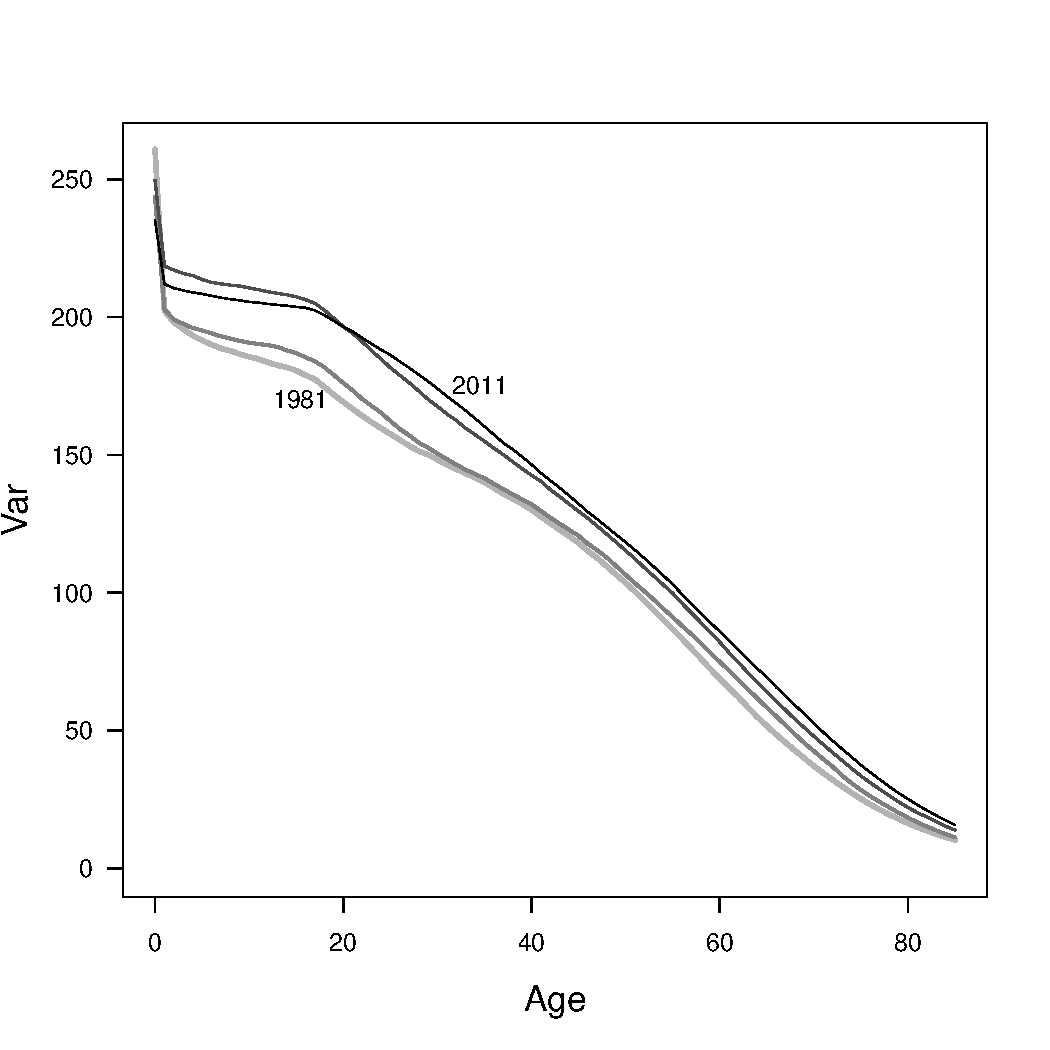
\includegraphics[width=\textwidth]{Figures/TotalVMales.pdf}
    \end{subfigure}%
    ~ 
    \begin{subfigure}[t]{0.5\textwidth}
        \centering
        \caption{Females}
        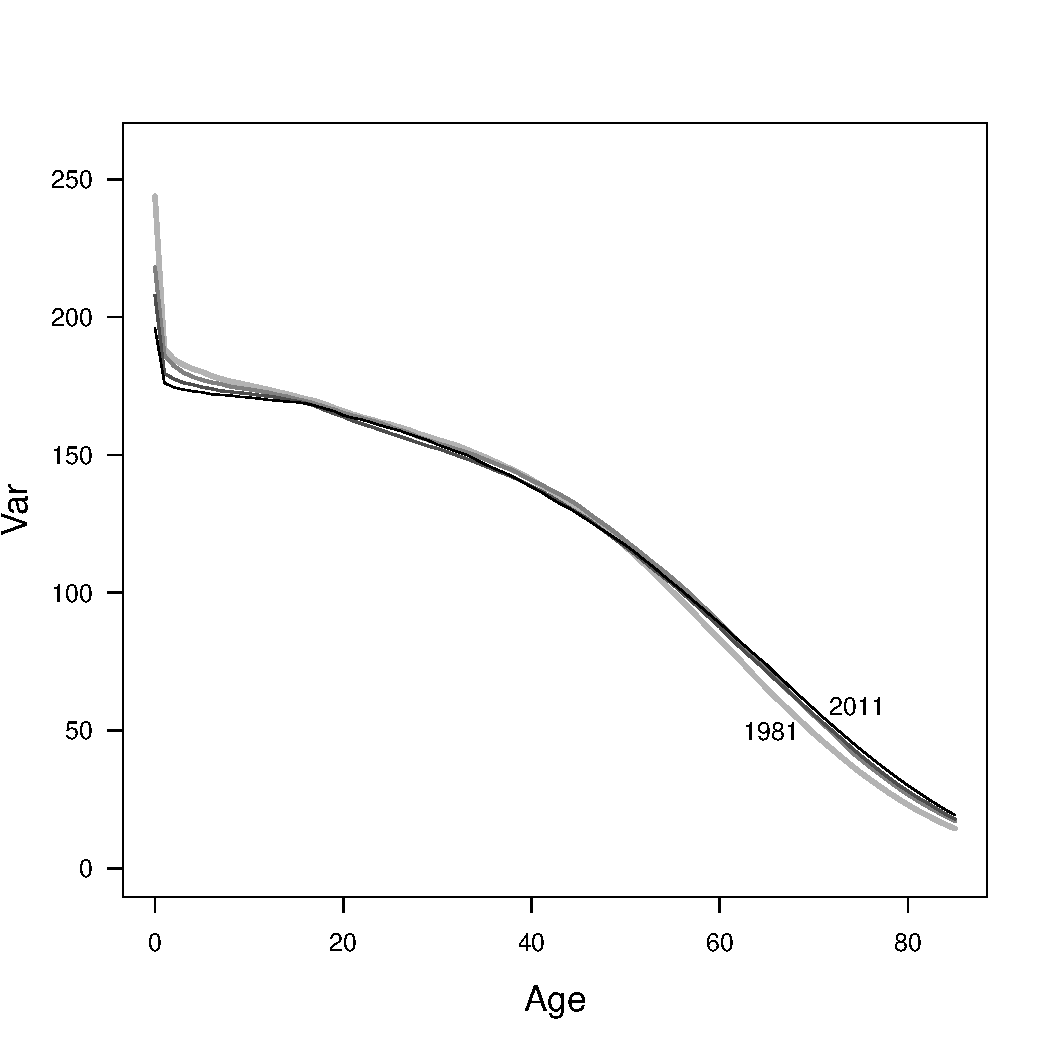
\includegraphics[width=\textwidth]{Figures/TotalVFemales.pdf}
    \end{subfigure}
\end{figure*}

\begin{figure*}[t!]
    \centering
      \caption{Standard deviation of remaining lifespan for total population by age, Census years
      1981 until 2011.}
      \label{fig:sdtotal}
    \begin{subfigure}[t]{0.5\textwidth}
        \centering
        \caption{Males}
        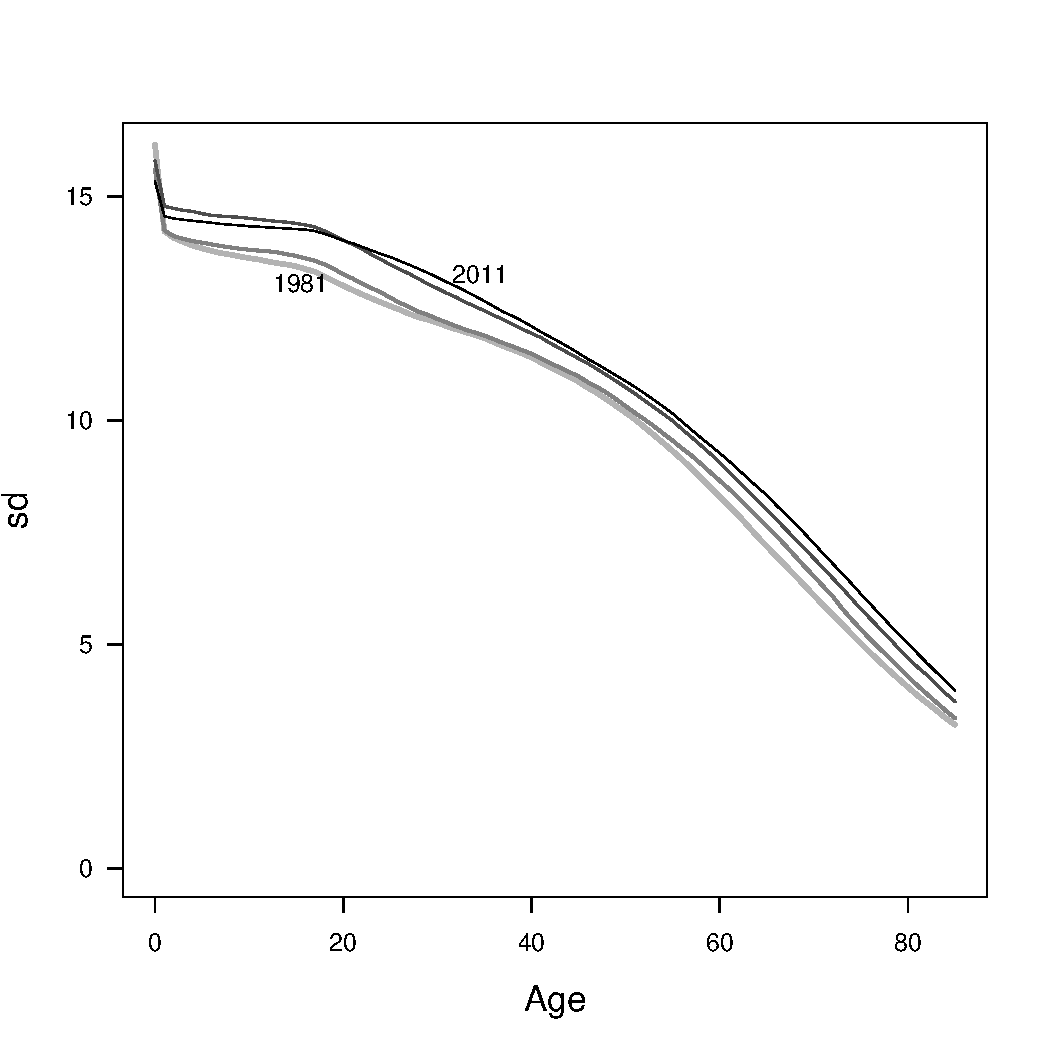
\includegraphics[width=\textwidth]{Figures/TotalsdMales.pdf}
    \end{subfigure}%
    ~ 
    \begin{subfigure}[t]{0.5\textwidth}
        \centering
        \caption{Females}
        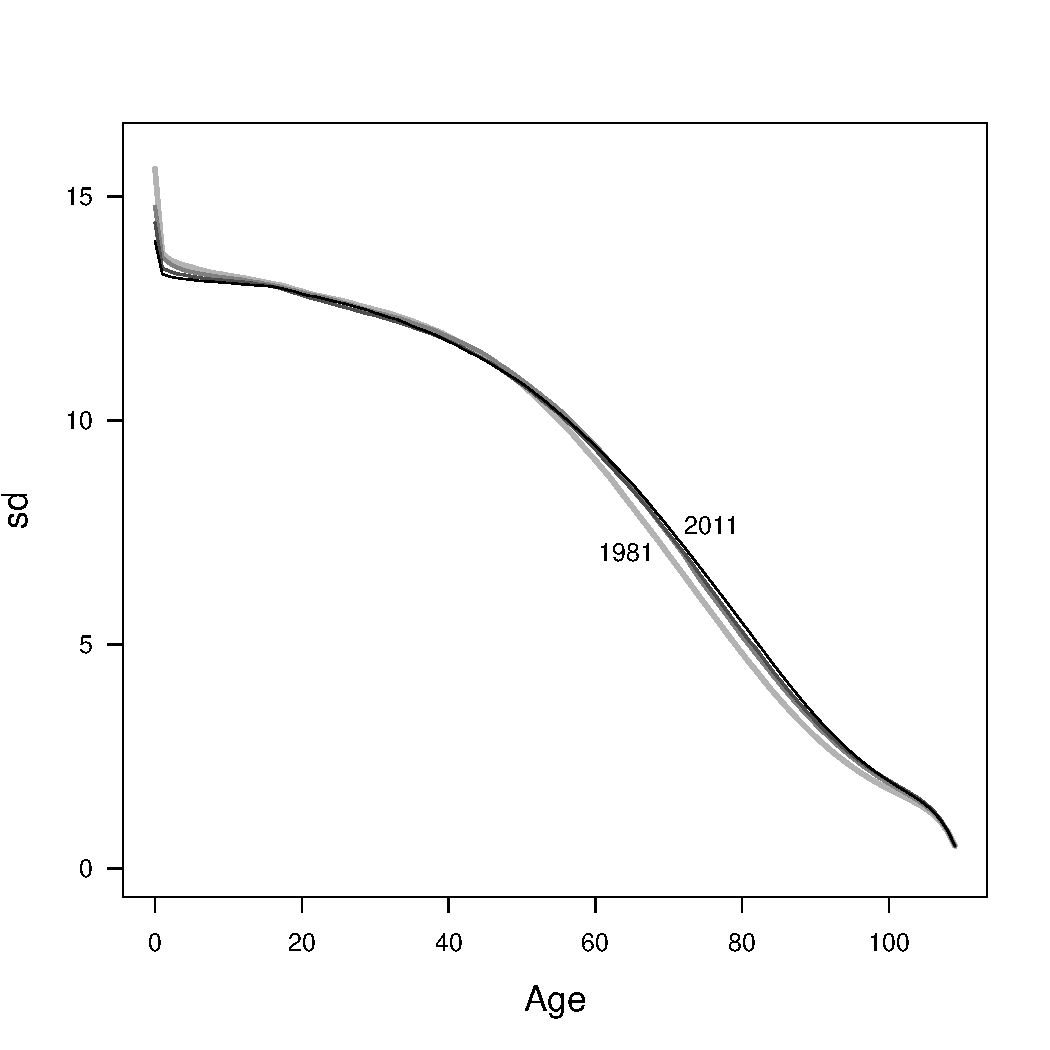
\includegraphics[width=\textwidth]{Figures/TotalsdFemales.pdf}
    \end{subfigure}
\end{figure*}

Figure~\ref{fig:decompmales} compares the proportion of the total difference in
variation in age at death that is due to between-group inequality with the proportion that is due to within-group variance. Figure~\ref{fig:decompfemales} shows the same for females. For males the proportion of variation explained by between-group inequality was lowest in 1981 and highest in 2001. By 2011 the proportion of between-group inequality had decreased slightly but was still greater than in 1981. The proportion of total variation in age at death explained by within-group variance was highest in 1981 and lowest in 2001. 
The proportion of variation explained by the within-group component increased slightly for males in 2011, which is mirrored in the decrease in the between-group component. This cross over between 2001 and 2011 was not found for females. For females the proportion explained by between-group inequality consistently increased between 1981 and was mirrored by a consistent decrease in the within-group component. Changes to the two components over time do not appear to have occurred across older ages for males or females. 


\begin{figure*}[t!]
    \centering
      \caption{Proportion of variance due to differences within and between deprivation
      quintiles by age, Census years 1981 until 2011, males.}
      \label{fig:decompmales}
    \begin{subfigure}[t]{0.5\textwidth}
        \centering
        \caption{Between}
        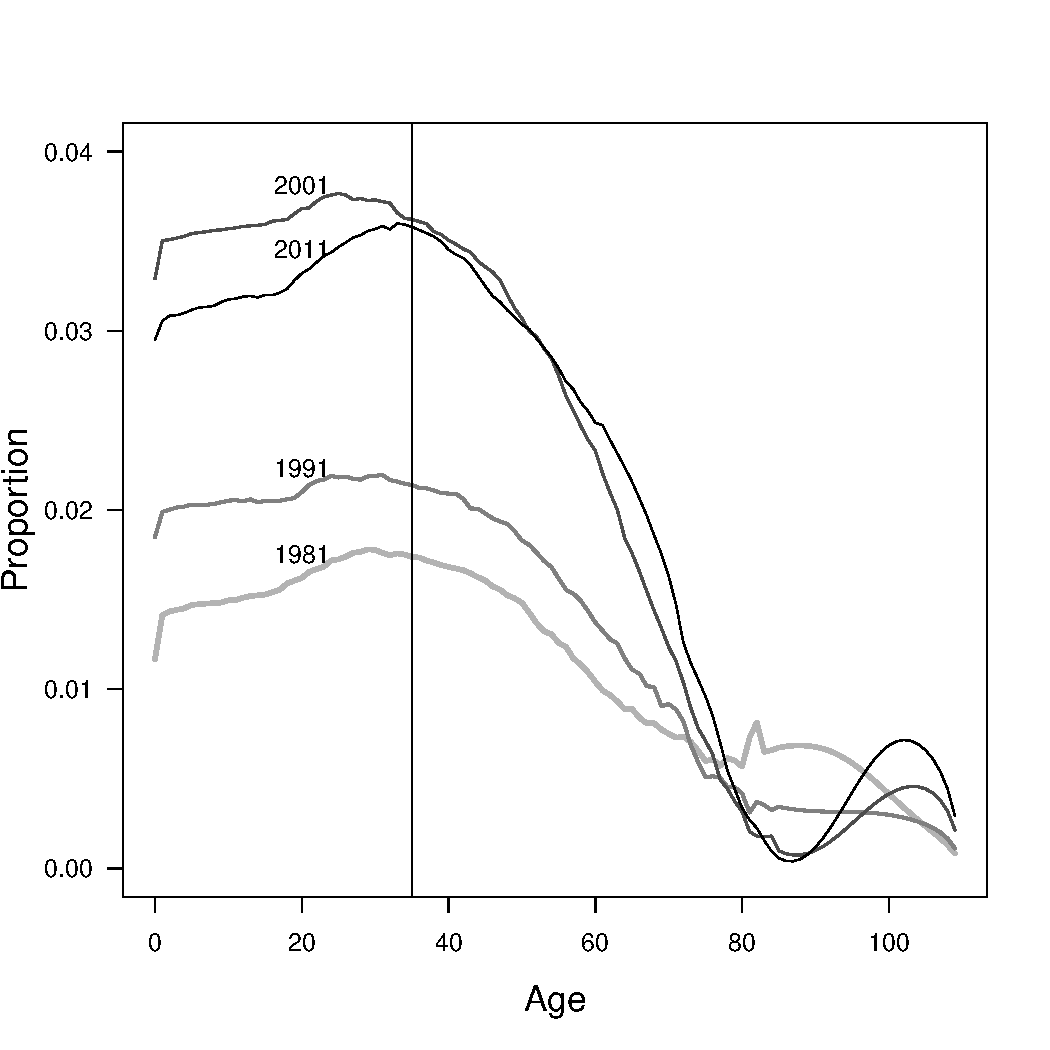
\includegraphics[width=\textwidth]{Figures/BetweenPropMales.pdf}
    \end{subfigure}%
    ~ 
    \begin{subfigure}[t]{0.5\textwidth}
        \centering
        \caption{Within}
        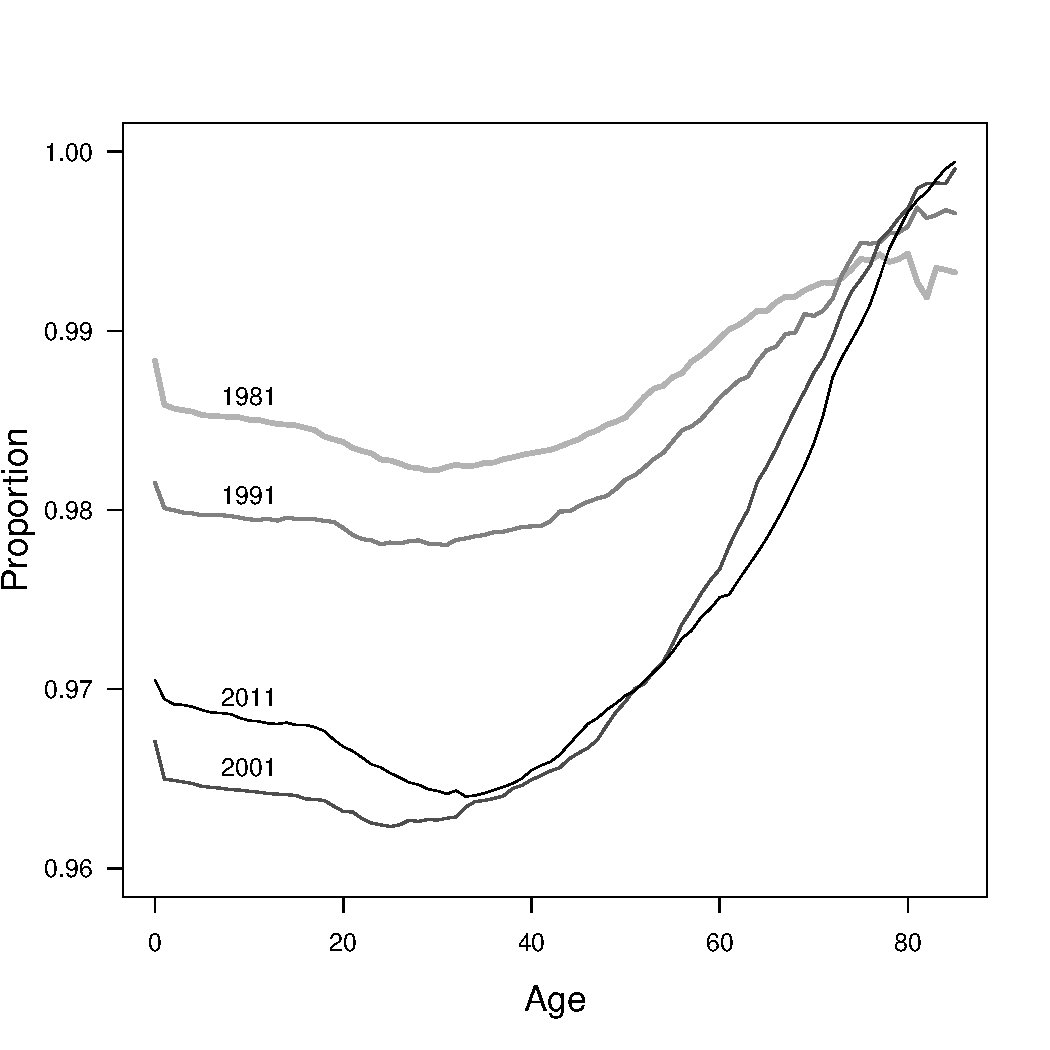
\includegraphics[width=\textwidth]{Figures/WithinPropMales.pdf}
    \end{subfigure}
\end{figure*}


\begin{figure*}[t!]
    \centering
      \caption{Proportion of variance due to differences between deprivation
      quintiles by age, Census years 1981 until 2011, females.}
      \label{fig:decompfemales}
    \begin{subfigure}[t]{0.5\textwidth}
        \centering
        \caption{Between}
        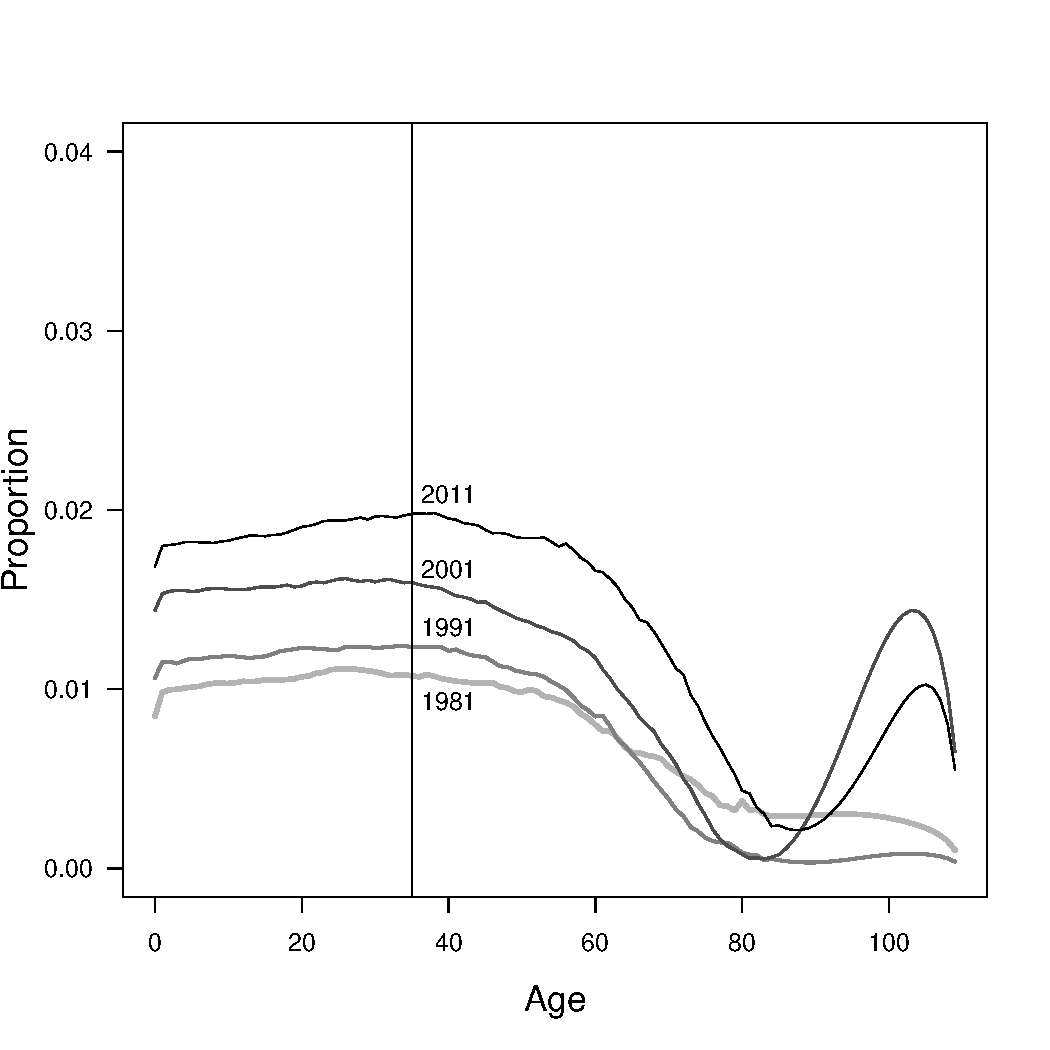
\includegraphics[width=\textwidth]{Figures/BetweenPropFemales.pdf}
    \end{subfigure}%
    ~ 
    \begin{subfigure}[t]{0.5\textwidth}
        \centering
        \caption{Within}
        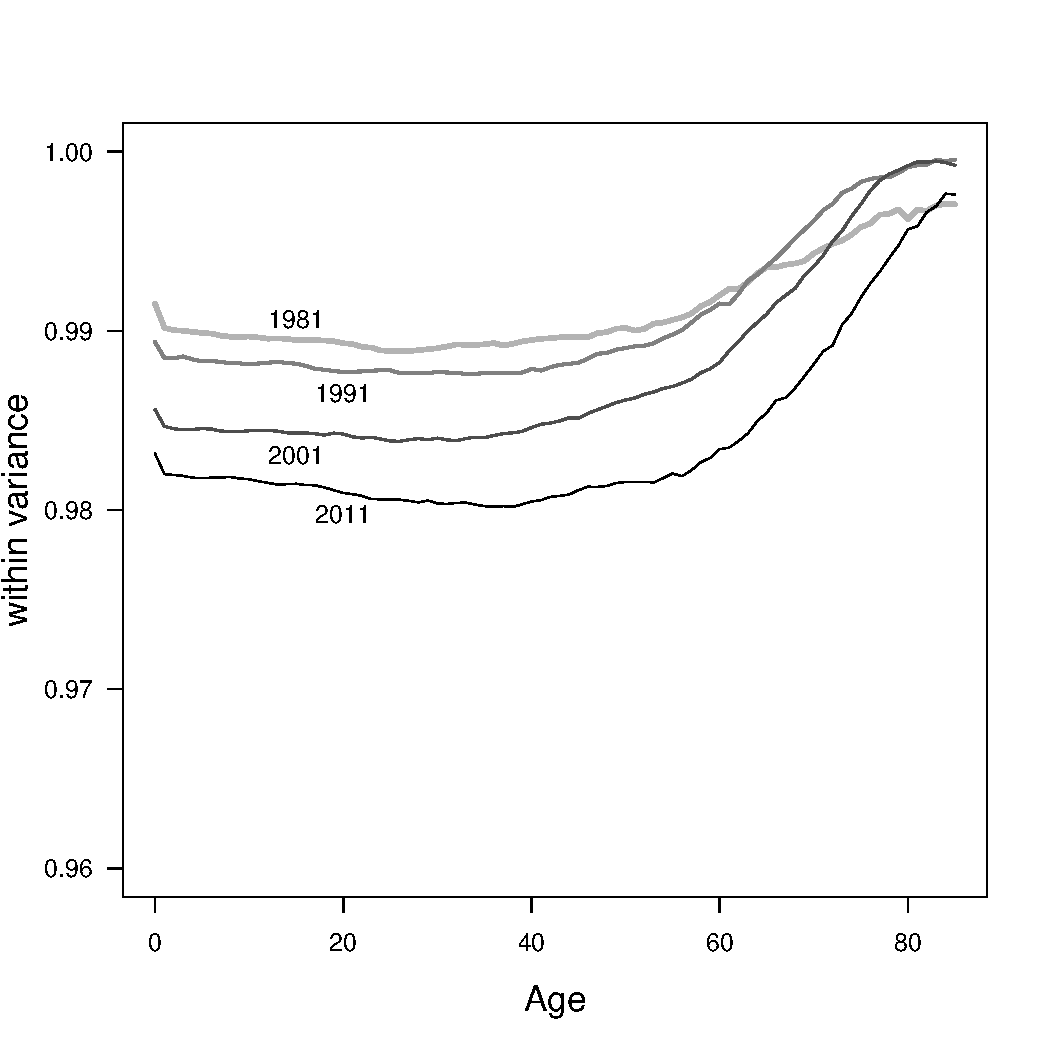
\includegraphics[width=\textwidth]{Figures/WithinPropFemales.pdf}
    \end{subfigure}
\end{figure*}


\FloatBarrier
\subsection{Sensitivity analysis}
We tested the sensitivity of our results to the size of deprivation group by
replicating the analysis using deciles of deprivation, each representing 10\% of
the population. The conclusions were the same for males and for females.
However, the increase in the between-group component over time was greater in
magnitude when using deciles. We chose to report results for quintiles of
deprivation as they are the preferred analytical grouping for routine reporting
of health measures in Scotland \citep{Health2017}.

\section{Discussion and conclusion}

\subsection{Summary of main findings}
Deprivation differences in age at death were evident at all Census years when measuring socioeconomic inequality by area-level. Those living in the most deprived areas can expect to live the shortest lives and experience the greatest variation in age at death: a double burden of mortality inequality. The difference between deprivation groups was larger for males than for females. Males from the most deprived quintile experienced increasing variation in age at death between 1991 and 2001 so that the level of variation in 2011 was the same as that experienced 30 years earlier. The proportion of variation in age at death explained by the between-group component of inequality was higher in 2011 than in 1981 for males and females.

\subsection{Strengths and limitations}
Our results are unable to determine the exact reason why the between-group proportion has increased. The timing of the increasing between-group component may be associated with the well documented 'polarization' of deprivation, health and mortality that increased in the UK following the 1980s \citep{Shaw2000,Mitchell2000} and they may provide support for existing theories which emphasizes the negative impact relative deprivation can have on population level health and mortality \citep{Wilkinson2007,Marmot2001}. Therefore our results are important for governments to consider when deciding how best to tackle mortality inequalities: whether to allocate resources to social policies that intervene at the contextual and area-level versus social policies that intervene at the individual level  \citep{Allik2016,Roux2001,Robert1999,TheScottishGovernment2016}. In addition to these theoretical contributions, our study demonstrates a number of empirical strengths.   

The data used for this study includes the most robust population estimates and mortality data for the entire population of Scotland. Using a validated area-level measure of socioeconomic inequality meant that complete lifetables could be constructed and no ages were truncated from the analysis. However, it is important to acknowledge the reasons why studies interested in the social distribution mechanisms of adult mortality may consider restricting analysis to older ages. \citet{Smits2009} suggest only looking at ages 15+ because these are the ages where 80\% of deaths in developed countries now occur. Looking only at adult mortality may better reflect the causes of death driving mortality change in more recent time periods: infectious disease and effective medical intervention historically reduced infant and childhood deaths rapidly but reductions in adult mortality are influenced by more complex mechanisms that change slowly \citep{Smits2009,Vallin2004}. Our results indicate that the age at which the difference in variation in age at death is greatest is around 35 years old. This provides some reassurance for studies that are forced to truncate out younger age groups: the peak of variation in age at death (at least in developed countries) is likely to be captured. 


The Carstairs score as an empirical measure has been critiqued. For example, the meaning of car ownership is fundamentally different for individuals in rural contexts compared to urban contexts. It is also acknowledged that overcrowding may occur out of choice and for cultural reasons rather than simply being a marker of deprivation \citep{Fischbacher2014}. Therefore it has been suggested that the Carstairs score may be an out of date measure of socioeconomic deprivation \citep{Schofield2016,Tunstall2011} because the relevance of the variables used for capturing the meaning of deprivation varies across contexts and over time \citep{Norman2010}. In response, it was demonstrated that the scores for each postcode sector at each Census year are highly correlated despite changes to the formal definitions of the variables. This is interpreted as evidence that the underlying information the variables aim to capture is similar or that deprivation has remained stable over time \citep{Leyland2007}. Alternative measures of area-level deprivation are available, for example the Scottish index of multiple deprivation (SIMD). The SIMD includes 38 indicators from 7 domains (employment,income,health,education,access to services, crime and housing). The SIMD was not suitable for the trend focus of this research as it is only recommended for analysis using data beginning in 1996 \citep{Health2017}. A further limitation is that it includes indicators of health and mortality meaning that the full SIMD can not be used for health inequalities research. Instead health inequalities research tends to use the income domain only \citep{Leyland2007a}. The income domain is highly correlated with the full SIMD and is one of the most heavily weighted domains \citep{Health2017,TheScottishGovernment2016}.   

\section{Conclusion}
Monitoring variance in age at death is complimentary to the routine monitoring of life expectancy: monitoring both allows us to establish if average population mortality and mortality inequalities have been improved simultaneously. This study has demonstrated increasing relative contributions from area-level deprivation differences to total variance in age at death using population level data for Scotland. This type of trend analysis is important for understanding the changing nature of the social determinants of mortality inequalities in developed countries.  More countries should begin to measure the between-group and within-group contributions to variance in age at death and monitor trends in order to understand the extent to which mortality is dependent upon, and amenable to, relative area-level deprivation.


\bibliographystyle{apalike}
\bibliography{references}

\section{Appendices}

\subsection{Appendix 1}
see supplementary pdf


\subsection{Appendix 2}

% Table generated by Excel2LaTeX from sheet 'Sheet1'
\begin{table}[htbp]
  \centering
  \caption{Life expectancy and standard deviation for males, age 35.}
    \begin{tabular}{lrrrrrrrr}
          & \multicolumn{2}{c}{1981} & \multicolumn{2}{c}{1991} & \multicolumn{2}{c}{2001} & \multicolumn{2}{c}{2011} \\
    \midrule
    quintile & \multicolumn{1}{c}{ex} & \multicolumn{1}{c}{sd} & \multicolumn{1}{c}{ex} & \multicolumn{1}{c}{sd} & \multicolumn{1}{c}{ex} & \multicolumn{1}{c}{sd} & \multicolumn{1}{c}{ex} & \multicolumn{1}{c}{sd} \\
    \midrule
    1 (least dep.) & 38.4  & 11.4  & 40.9  & 11.2  & 43.7  & 11.3  & 46.3  & 11.1 \\
    2     & 37.1  & 11.6  & 39.5  & 11.6  & 41.9  & 11.8  & 44.7  & 12.0 \\
    3     & 36.4  & 11.8  & 38.8  & 11.8  & 40.5  & 12.2  & 43.4  & 12.4 \\
    4     & 35.5  & 11.8  & 37.6  & 11.9  & 39.1  & 12.5  & 41.7  & 13.0 \\
    5 (most dep.) & 33.8  & 12.1  & 35.8  & 12.3  & 36.6  & 13.2  & 39.2  & 13.5 \\
    Total pop. & 36.2  & 11.8  & 38.5  & 11.8  & 40.3  & 12.4  & 43.1  & 12.6 \\
    \bottomrule
    \end{tabular}%
  \label{tab:addlabel}%
\end{table}%

\subsection{Appendix 3}
% Table generated by Excel2LaTeX from sheet 'Sheet1'
\begin{table}[htbp]
  \centering
  \caption{Life expectancy and standard deviation for females, age 35.}
    \begin{tabular}{lrrrrrrrr}
          & \multicolumn{2}{c}{1981} & \multicolumn{2}{c}{1991} & \multicolumn{2}{c}{2001} & \multicolumn{2}{c}{2011} \\
    \midrule
    quintile & \multicolumn{1}{c}{ex} & \multicolumn{1}{c}{sd} & \multicolumn{1}{c}{ex} & \multicolumn{1}{c}{sd} & \multicolumn{1}{c}{ex} & \multicolumn{1}{c}{sd} & \multicolumn{1}{c}{ex} & \multicolumn{1}{c}{sd} \\
    \midrule
    1 (least dep.) & 43.4  & 11.7  & 45.1  & 11.5  & 47.0  & 11.1  & 49.0  & 49.0 \\
    2     & 42.2  & 12.0  & 44.4  & 11.7  & 46.1  & 11.5  & 47.9  & 47.9 \\
    3     & 41.6  & 12.2  & 43.8  & 12.1  & 45.0  & 12.0  & 46.7  & 46.7 \\
    4     & 41.0  & 12.1  & 42.7  & 12.3  & 44.1  & 12.2  & 45.7  & 45.7 \\
    5 (most dep.) & 39.6  & 12.7  & 41.4  & 12.8  & 42.6  & 13.1  & 43.9  & 43.9 \\
    Total pop. & 41.5  & 12.2  & 43.4  & 12.2  & 44.9  & 12.1  & 46.7  & 46.7 \\
    \bottomrule
    \end{tabular}%
  \label{tab:addlabel}%
\end{table}%


\end{document}